\begin{figure}[htp]
\centering
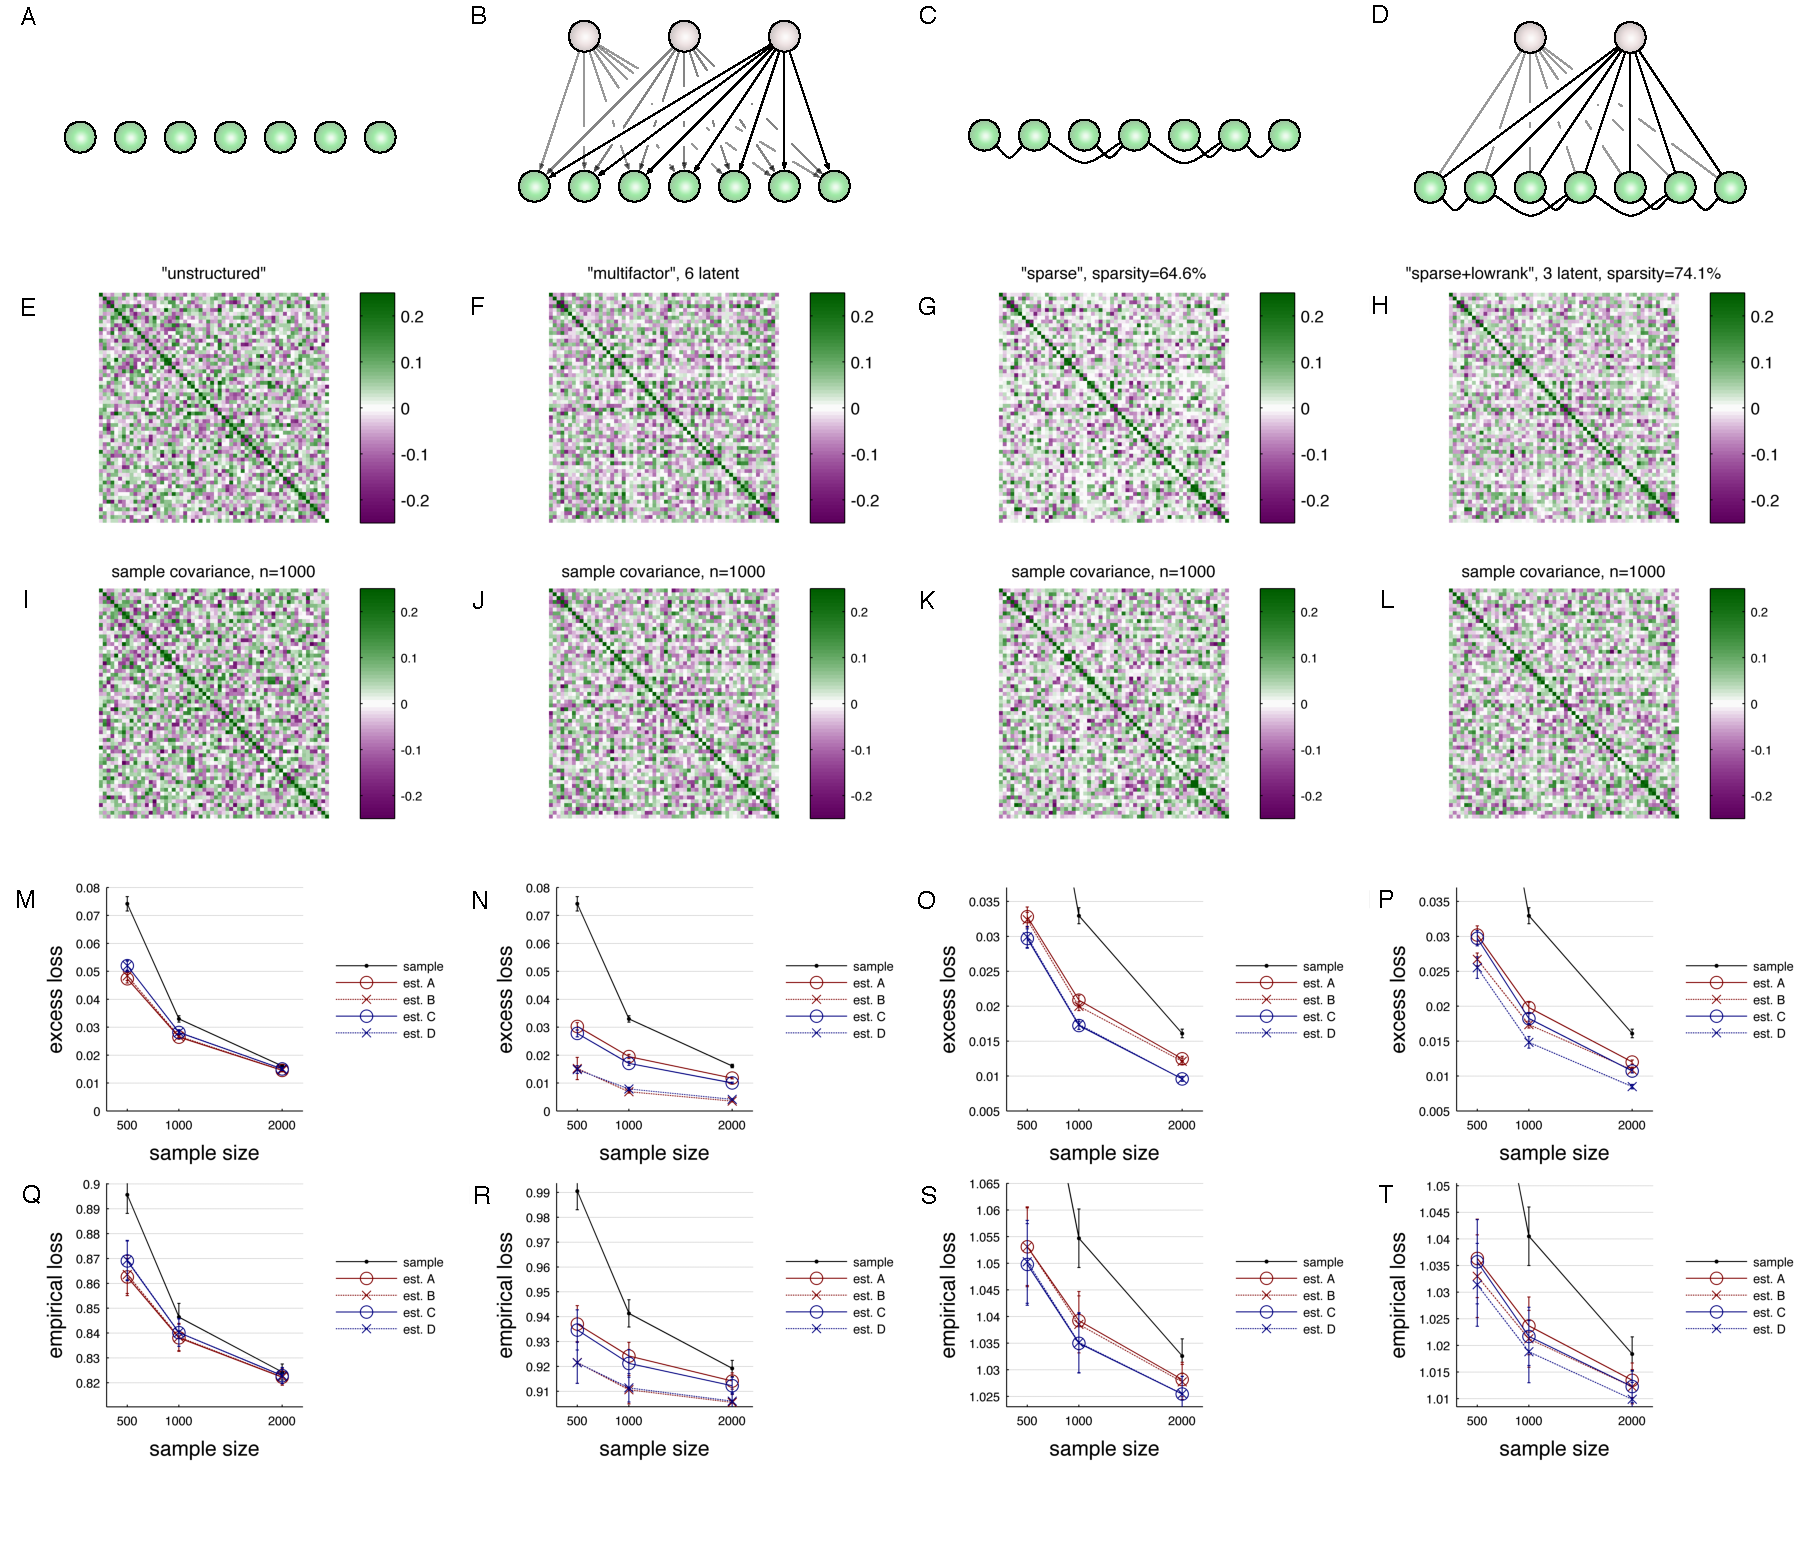
\includegraphics[width=1.0\textwidth]{figures/Figure3.pdf}
\caption{
In simulation, selection amongst estimators recognizes the true covariance atructure. 
{\bf A--D} are examples of true $100\times100$ covariance matrices of multivariate normal distributions used in simulations. Matrix A has no low-dimensional structure. Matrices B--D have low-dimensional structture corresponding to the respective graphical models in Fig.~2B--D.
{\bf E--H} are examples of sample covariance matrices obtained from samples of size $n=1000$ from distributions with respective true covariance matrices A--D.
{\bf I--L:} Performance evaluation of covariance estimators A, B, C, D from samples obtained from models A, B, C, D.  Excess loss $\loss{\hat\Sigma,\Sigma}-\loss{\Sigma,\Sigma}$ is only accessible with the true covariance matrix $\Sigma$ is known and zero excess loss implies absolutely correct estimation. Estimators that can represent the graphical model outperform those that cannot.  Error bars indicate the standard deviation. 
{\bf M--P:} Performance evaluation using \emph{validated loss} from Eq.~\ref{eq:validationLoss} without knowledge of true $\Sigma$. Cross-validation reproduces the same relationship between performances of the estimators.
}\label{fig:03}
\end{figure}